% CVPR 2022 Paper Template
% based on the CVPR template provided by Ming-Ming Cheng (https://github.com/MCG-NKU/CVPR_Template)
% modified and extended by Stefan Roth (stefan.roth@NOSPAMtu-darmstadt.de)

\documentclass[10pt,twocolumn,letterpaper]{article}

%%%%%%%%% PAPER TYPE  - PLEASE UPDATE FOR FINAL VERSION
%\usepackage[review]{cvpr}      % To produce the REVIEW version
\usepackage{cvpr}              % To produce the CAMERA-READY version
%\usepackage[pagenumbers]{cvpr} % To force page numbers, e.g. for an arXiv version

% Include other packages here, before hyperref.
\usepackage{graphicx}
\usepackage{amsmath}
\usepackage{amssymb}
\usepackage{booktabs}
\usepackage{tikz}
\usetikzlibrary{shapes.geometric, arrows.meta, positioning, fit, backgrounds}

\newcommand{\latex}{\LaTeX\xspace}
\newcommand{\tex}{\TeX\xspace}


% It is strongly recommended to use hyperref, especially for the review version.
% hyperref with option pagebackref eases the reviewers' job.
% Please disable hyperref *only* if you encounter grave issues, e.g. with the
% file validation for the camera-ready version.
%
% If you comment hyperref and then uncomment it, you should delete
% ReviewTempalte.aux before re-running LaTeX.
% (Or just hit 'q' on the first LaTeX run, let it finish, and you
%  should be clear).
\usepackage[pagebackref,breaklinks,colorlinks]{hyperref}


% Support for easy cross-referencing
\usepackage[capitalize]{cleveref}
\crefname{section}{Sec.}{Secs.}
\Crefname{section}{Section}{Sections}
\Crefname{table}{Table}{Tables}
\crefname{table}{Tab.}{Tabs.}

\begin{document}

%%%%%%%%% TÍTULO

\title{Detección y Clasificación de Patógenos Foliares mediante Visión por Computador}

\author{
   Gabriel Sánchez Muñoz\\{\tt\small gabrielsm@correo.ugr.es}
   \and
   Germán Rodríguez Vidal\\{\tt\small germanrv@correo.ugr.es}
   \and
   Pablo García Bas\\{\tt\small pablogb@correo.ugr.es}
   \and
   Miguel Ángel Moreno Castro\\{\tt\small miguelangelmc@correo.ugr.es}
}

\maketitle

%%%%%%%%% RESUMEN
\begin{abstract}
   La detección temprana y precisa de enfermedades vegetales es crítica para la agricultura de precisión y la seguridad alimentaria.
   Los enfoques actuales basados en Deep Learning, a pesar de mostrar resultados prometedores, suelen carecer de información contextual sobre el huésped, lo que limita su precisión en escenarios de múltiples cultivos. 
   Este trabajo propone un enfoque jerárquico de dos etapas para abordar esta limitación. En primer lugar, se realiza una clasificación de la especie arbórea para establecer un contexto biológico y, posteriormente, un detector de objetos localiza y clasifica los patógenos específicos asociados a dicha especie.
   Los resultados muestran que incorporar la identificación previa del huésped incrementa la precisión media (mAP) en un [X]\% respecto a los detectores genéricos de una sola etapa ("end-to-end"), demostrando la superioridad de los modelos condicionados biológicamente.
\end{abstract}

%%%%%%%%% CUERPO DEL TEXTO
\section{Introducción}
\label{sec:intro}
Las enfermedades de las plantas representan una amenaza significativa para la seguridad alimentaria mundial y la estabilidad económica agrícola, causando pérdidas estimadas de hasta el 30\% en el rendimiento de los cultivos cada año \cite{savary2019global}. 
La identificación temprana y precisa de estas patologías es crucial para aplicar medidas de control eficaces y minimizar el uso de químicos. 
Tradicionalmente, este diagnóstico ha dependido de la inspección visual manual por parte de expertos, un proceso que resulta laborioso, subjetivo y difícil de escalar a grandes explotaciones \cite{barbedo2013digital}.

En la última década, la visión por computador y, específicamente, el aprendizaje profundo, han emergido como herramientas poderosas para automatizar esta tarea. 
El uso de Redes Neuronales Convolucionales (CNNs) ha permitido grandes avances tanto en la clasificación de imágenes (identificar si una hoja está enferma) como en la detección de objetos (localizar la lesión exacta en la hoja) \cite{mohanty2016using}. 
Sin embargo, la mayoría de las arquitecturas actuales abordan la detección de enfermedades como un problema monolítico donde los modelos se entrenan para detectar cualquier enfermedad en cualquier tipo de hoja simultáneamente, ignorando a menudo la estructura jerárquica natural de la taxonomía biológica.

Debido a que muchas patologías foliares comparten características visuales similares, independientemente de la especie, los detectores agnósticos al huésped sufren de una alta confusión inter-clase. 
Esto suele derivar en predicciones erróneas donde se asocian enfermedades a plantas incompatibles, reduciendo la precisión y confiabilidad del sistema en aplicaciones del mundo real.

Para resolver esto, proponemos un enfoque jerárquico que imita el diagnóstico experto donde primero se identifica la especie del árbol para simplificar la búsqueda de la enfermedad y luego se aplica un detector especializado para esa especie.

\section{Dataset}

Para validar nuestro enfoque jerárquico, hemos confeccionado un \textit{dataset} que integra imágenes de tres cultivos: rosa, patata y manzana. 
Las imágenes provienen de la plataforma Roboflow Universe, que contiene una gran cantidad de \textit{datasets} de código abierto, y han sido seleccionadas por su calidad y variedad de condiciones de iluminación.

\begin{itemize}
   \item Rose Dataset: Consta de 2,725 imágenes y abarca 4 clases (Black Spot, Downy Mildew, Powdery Mildew y hojas sanas).
   \item Potato Dataset: Comprende 812 imágenes distribuidas en [X] clases (típicamente Early Blight, Late Blight, Healthy).
   \item Apple Dataset: Incluye 1582 imágenes que cubren 4 patologías (Alternaria Spot, Brown Spot, Gray Spot, Rust).
\end{itemize}

El dataset combinado se dividió aleatoriamente en subconjuntos de Entrenamiento (70\%), Validación (15\%) y Prueba (15\%), preservando la estratificación de clases para garantizar una evaluación equilibrada.

\section{Clasificación}

Para el diseño del módulo de clasificación, hemos evaluado dos paradigmas principales del estado del arte, las arquitecturas basadas en Vision Transformers (ViT) y las Redes Neuronales Convolucionales (CNNs). 
Nuestro objetivo fue contrastar la capacidad de modelado global de los Transformers frente a la eficiencia inductiva de las CNNs. 
Adicionalmente, dada la orientación práctica de este proyecto hacia una futura aplicación móvil, se incluyó en el estudio un modelo diseñado específicamente para entornos de recursos limitados.

\subsection{MaxViT}

Dentro de la familia de los Transformers, MaxViT (Multi-Axis Vision Transformer) combina tanto mecanismos de atención global como convoluciones locales para capturar características a múltiples escalas \cite{tu2022maxvit}.
Su característica distintiva es el mecanismo de \textit{Multi-Axis Self-Attention} (Max-SA), que descompone el cálculo de atención en dos operaciones: atención local (\textit{Block Attention}) para capturar texturas finas, y atención global dispersa (\textit{Grid Attention}) para relacionar partes distantes de la imagen.

\subsubsection{EfficientNetV2}

Esta arquitectura mejora a su predecesora mediante la introducción de bloques Fused-MBConv \cite{tan2021efficientnetv2}.
Estos bloques reemplazan las convoluciones \textit{depthwise} separables tradicionales por convoluciones estándar $3 \times 3$ fusionadas en las primeras capas.

\subsection{MobileNet}

La base de su eficiencia radica en las convoluciones \textit{depthwise} separables, que factorizan la operación de convolución estándar en dos capas más ligeras (profundidad y punto a punto), reduciendo drásticamente la cantidad de parámetros y operaciones \cite{howard2017mobilenets}. 
Aunque su capacidad de representación es menor que los modelos anteriores, su inclusión es crítica para evaluar el compromiso (\textit{trade-off}) entre precisión y latencia en una aplicación real para agricultores.

\section{Detección de Objetos}

El objetivo fundamental en detección de objetos es localizar y clasificar regiones de interés (\textit{bounding boxes}). 
Históricamente, métodos dominantes como \textit{Deformable Parts Model} (DPM) abordaban este problema mediante un enfoque de ventana deslizante (\textit{sliding window}) que resultaban inviables computacionalmente al procesar todas las posibles sub-ventanas \cite{felzenszwalb2010dpm}.

La evolución comenzó con \textbf{R-CNN}, un modelo de 3 etapas donde una búsqueda selectiva genera regiones potencialmente interesantes, una CNN extrae características y un SVM las clasifica \cite{girshick2014rcnn}. 
Sus limitaciones principales son el alto coste de procesar regiones por separado y la falta de aprendizaje en la búsqueda selectiva. 

\subsection{Faster R-CNN}

Faster R-CNN integra la propuesta de regiones dentro de la red neuronal, reemplazando el algoritmo fijo por una \textit{Region Proposal Network} (RPN) entrenable y más rápida \cite{ren2016fasterrcnn}. 

En primer lugar se definen \textit{anchor points} sobre el mapa de características de la imagen, actuando como centros de posibles regiones con diferentes escalas y ratios. Seguidamente, la RPN predice simultáneamente la probabilidad de objeto y las coordenadas del \textit{bounding box}.

A pesar de su alta precisión, el hecho de ser un modelo de dos etapas penaliza su velocidad de inferencia.
\subsection{YOLO}

Como respuesta a la latencia, \textit{You Only Look Once} (YOLO) redefinió la detección no como una clasificación de regiones, sino como un problema único de regresión, descartando por completo el pipeline disjunto de DPM y R-CNN.

YOLO utiliza una única red neuronal convolucional que procesa la imagen completa de una sola vez.
Divide la imagen en una cuadrícula ($S \times S$) donde cada celda predice $B$ bounding boxes y sus respectivas puntuaciones de confianza.

La arquitectura unificada de YOLO permite una inferencia en tiempo real inalcanzable para los métodos de dos etapas \cite{redmon2016yolo}. Mientras que Faster R-CNN procesa aproximadamente 0.5 FPS, YOLO alcanza los 45 FPS, ofreciendo la inmediatez necesaria para aplicaciones agrícolas prácticas.
\section{Métodos}
\label{sec:metodos}

En esta sección se detalla la propuesta arquitectónica diseñada para la detección de patologías foliares. El sistema se fundamenta en un enfoque jerárquico de dos etapas, compuesto secuencialmente por un módulo de clasificación taxonómica (especie vegetal) y un módulo de detección de objetos (patógeno y localización dentro de la imagen).


\subsection{Arquitectura del Pipeline Propuesto}

\begin{figure*}[t] % El asterisco hace que ocupe el ancho de las dos columnas
\centering
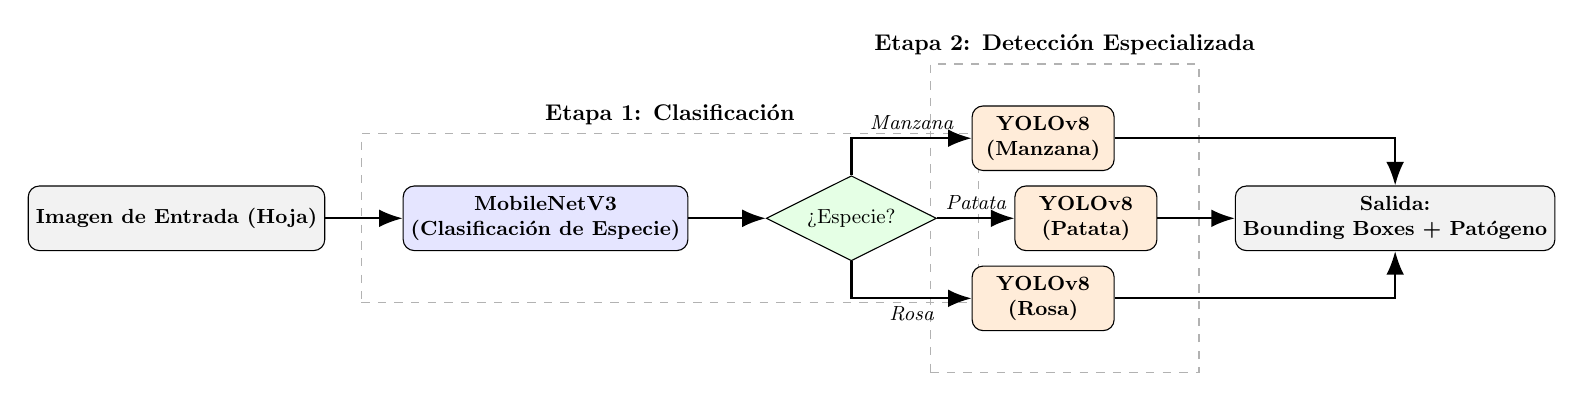
\begin{tikzpicture}[
    scale=0.82, transform shape,
    node distance=1.2cm and 1.2cm,
    box/.style={draw, rectangle, rounded corners, minimum width=2.8cm, minimum height=1cm, text centered, align=center, font=\bfseries\small, fill=blue!10},
    yolo/.style={draw, rectangle, rounded corners, minimum width=2.2cm, minimum height=1cm, text centered, align=center, font=\bfseries\small, fill=orange!15},
    decision/.style={draw, diamond, aspect=2, minimum width=2.2cm, minimum height=1cm, text centered, align=center, font=\small, fill=green!10},
    arrow/.style={-{Latex[length=3mm]}, thick},
    label_text/.style={font=\small\itshape}
]

% Nodos principales
\node (input) [box, fill=gray!10] {Imagen de Entrada (Hoja)};

% Etapa 1: Clasificación
\node (mobilenet) [box, right=of input] {MobileNetV3\\(Clasificación de Especie)};

% Decisión
\node (switch) [decision, right=of mobilenet] {¿Especie?};

% Etapa 2: Detección (YOLOv8)
\node (yolo_apple) [yolo, above right=0.4cm and 1.2cm of switch] {YOLOv8\\(Manzana)};
\node (yolo_potato) [yolo, right=1.2cm of switch] {YOLOv8\\(Patata)};
\node (yolo_rose) [yolo, below right=0.4cm and 1.2cm of switch] {YOLOv8\\(Rosa)};

% Salida
\node (output) [box, fill=gray!10, right=of yolo_potato] {Salida:\\Bounding Boxes + Patógeno};

% Conexiones
\draw [arrow] (input) -- (mobilenet);
\draw [arrow] (mobilenet) -- (switch);

% Flechas del switch a los YOLOs
\draw [arrow] (switch.north) |- (yolo_apple.west) node[pos=0.75, above, label_text] {Manzana};
\draw [arrow] (switch.east) -- (yolo_potato.west) node[midway, above, label_text] {Patata};
\draw [arrow] (switch.south) |- (yolo_rose.west) node[pos=0.75, below, label_text] {Rosa};

% Flechas de los YOLOs a la salida
\draw [arrow] (yolo_apple.east) -| (output.north);
\draw [arrow] (yolo_potato.east) -- (output.west);
\draw [arrow] (yolo_rose.east) -| (output.south);

% Recuadro de fondo (opcional para agrupar las etapas)
\begin{scope}[on background layer]
    \node [draw=black!30, dashed, fit=(mobilenet) (switch), inner sep=15pt, label=above:{\textbf{Etapa 1: Clasificación}}] {};
    \node [draw=black!30, dashed, fit=(yolo_apple) (yolo_potato) (yolo_rose), inner sep=15pt, label=above:{\textbf{Etapa 2: Detección Especializada}}] {};
\end{scope}

\end{tikzpicture}
\caption{Visión general de la arquitectura jerárquica propuesta. Una imagen de entrada es procesada primero por una red MobileNetV3 para identificar el cultivo huésped (Etapa 1). En base a esta predicción, se selecciona dinámicamente un modelo de detección YOLOv8 especializado (Etapa 2) para localizar y clasificar las patologías foliares correspondientes, evitando la confusión inter-especie.}
\label{fig:pipeline}
\end{figure*}

Para evaluar la eficacia del condicionamiento biológico en la detección de enfermedades, se implementaron y compararon tres variantes arquitectónicas del pipeline. Todas comparten la etapa inicial de clasificación, pero difieren en la estrategia de detección posterior:

\begin{itemize}
    \item \textbf{V1: Arquitectura de Expertos Especializados (Ramificada).} En este esquema, la predicción del clasificador actúa como un enrutador (\textit{router}). Dependiendo de la especie predicha, la imagen se deriva a uno de los tres detectores YOLO independientes, cada uno entrenado exclusivamente con el subconjunto de datos de dicha especie (Rosa, Patata o Manzana). Esto elimina la confusión inter-clase de especies a nivel de detector.
    
    \item \textbf{V2: Arquitectura Secuencial Global (Baseline).} El clasificador identifica la especie para aportar contexto, pero la detección se realiza mediante un único modelo YOLO global entrenado con el dataset completo (todas las clases de patógenos y especies simultáneamente). Este enfoque evalúa si la especialización (modelo V1) es realmente necesaria frente a un detector robusto generalista (modelo V2).
    
    \item \textbf{V3: Arquitectura Global Condicionada.} Una variante híbrida donde se utiliza un único detector global, pero la salida del clasificador se utiliza para filtrar o condicionar las predicciones del detector (e.g., penalizando la confianza de patógenos incompatibles con la especie detectada).
\end{itemize}

\subsection{Selección del Clasificador: MobileNet}

De los modelos evaluados en la fase preliminar (MaxViT, EfficientNetV2 y MobileNet), se seleccionó \textbf{MobileNet} \cite{howard2017mobilenets} como el extractor de características para la primera etapa.

Esta decisión se justifica por el \textit{trade-off} entre precisión y coste computacional. Los experimentos mostraron que, dada la baja cardinalidad del problema de clasificación (únicamente 3 clases: rosa, patata, manzana), modelos de alta capacidad como MaxViT no aportaban una ganancia significativa de precisión (saturación de rendimiento), mientras que introducían una latencia considerable. MobileNet, gracias a sus convoluciones separables en profundidad (\textit{depthwise separable convolutions}), ofrece un rendimiento competitivo con una fracción de los parámetros, alineándose con el objetivo de despliegue en dispositivos móviles.


\subsection{Selección del Detector: YOLOv8}

Para la etapa de localización de patógenos, se realizó una comparativa entre detectores de dos etapas (\textbf{Faster R-CNN}) y de una etapa (\textbf{YOLO}). Finalmente, se optó por la arquitectura \textbf{YOLOv8}, específicamente la variante \textit{small} (YOLOv8s).

La elección se fundamenta en dos factores críticos observados durante la experimentación:

\begin{enumerate}
    \item \textbf{Generalización y Convergencia:} Faster R-CNN mostró una tendencia al sobreajuste (\textit{overfitting}) temprano con nuestro dataset, degradando su rendimiento en el conjunto de test en comparación con YOLO bajo el mismo número de épocas de entrenamiento.
    \item \textbf{Eficiencia de Inferencia:} Como se discutió en la introducción, la aplicabilidad en campo requiere tiempos de respuesta rápidos. YOLOv8s, al ser un detector \textit{single-stage} libre de la red de propuesta de regiones (RPN), demostró una velocidad de inferencia (FPS) muy superior, esencial para la experiencia de usuario en tiempo real.
\end{enumerate}

Finalmente, la elección de la arquitectura se acotó a dos candidatos (si bien en las pruebas se consideraron hasta 8 versiones distintas de YOLO): \textbf{YOLOv8s} y la reciente versión \textbf{YOLO11s}. Aunque ambos modelos mostraron un desempeño sobresaliente, la balanza se inclinó a favor de YOLOv8s por dos razones fundamentales:

\begin{enumerate}
    \item \textbf{Consistencia en la precisión:} YOLOv8s demostró una mayor robustez inter-dominio. Superó a YOLO11s en el dataset de rosas con un margen de $+1.5\%$ de mAP y mantuvo un empate técnico en patatas, mientras que la ventaja de YOLO11s en manzanas fue marginal ($<0.3\%$), no compensando su inestabilidad en otros escenarios.
    
    \item \textbf{Eficiencia computacional:} Se observó un patrón constante de mayor eficiencia en la versión 8. YOLOv8s no solo requirió menores tiempos de entrenamiento para converger (e.g., $14.1$ min vs $16.8$ min en rosas), sino que, críticamente, ofreció una latencia de inferencia menor ($2.66$ img/s frente a $2.50$ img/s de la v11s). Esta ganancia del $6.4\%$ en velocidad es determinante para el despliegue en tiempo real propuesto.
\end{enumerate}

En consecuencia, se selecciona \textbf{YOLOv8s} como el detector final, al ofrecer el mejor equilibrio entre estabilidad predictiva y agilidad de procesamiento.


\section{Experimentos}

Para la elección del mejor metodo para detección y clasificación de patógenos foliares, se ha utilizado el conjunto de datos Global Plant Dataset, un corpus heterogéneo , compuesto por los anteriores datsets mencionados , con ellos se han realizado diversos experimentos. A continuación se describen los experimentos realizados y los resultados obtenidos.\\

\subsection{Metricas de Evaluación}
Para la evaluación de los modelos de clasificación, se han utilizado las métricas de precisión, mAP 50 y mAP 50-95. La precisión mide la proporción de predicciones correctas sobre el total de predicciones realizadas. El mAP 50 (mean Average Precision at IoU 0.5) evalúa la precisión promedio considerando un umbral de Intersección sobre Unión (IoU) del 50\%, mientras que el mAP 50-95 promedia la precisión en múltiples umbrales de IoU, proporcionando una evaluación más robusta del rendimiento del modelo.\\

Se diseñaron tres experimentos principales para comparar los enfoques de detección y clasificación:\\

\subsection{Arquitecturas del pipeline implementadas}
El primer  experimento (Baseline Monolitico) consiste en entrenar un único modelo de detección de objetos (YOLOv8) para identificar todas las clases de patógenos foliares sin considerar la especie del árbol huésped. Este modelo debe distinguir simultáneamente entre todas las enfermedades de todas las plantas, representando el enfoque estándar "end-to-end". Este enfoque sirve como línea base para evaluar la efectividad de los métodos jerárquicos.\\

El segundo experimento (Pipeline Híbrido Unificado)  implementa un enfoque jerárquico en dos etapas. En la primera etapa, se entrenó un modelo de clasificación de imágenes basado en MobileNet para identificar la especie del árbol (rosa, patata o manzana), alcanzando una exactitud del 99.84\%. En la segunda etapa, la predicción de la especie actúa como un mecanismo de condicionamiento lógico (masking) sobre un único detector YOLOv8, restringiendo el espacio de búsqueda exclusivamente a las enfermedades biológicamente plausibles para la especie identificada. Este enfoque permite reducir drásticamente las confusiones entre especies sin incrementar significativamente el coste computacional.

El tercer experimento (Pipeline Híbrico Modular)  explora una arquitectura jerárquica aún más especializada. Tras la clasificación de la especie vegetal mediante MobileNet, se activan modelos de detección independientes entrenados específicamente para cada especie. Cada detector se enfoca únicamente en distinguir entre los distintos patógenos foliares asociados a una única planta hospedadora. Este diseño maximiza la especialización del modelo y minimiza la ambigüedad inter-especie.


\begin{table*}[!t]
\centering
\caption{Comparativa de rendimiento (mAP@50 y mAP@50-95).}
\label{tab:resultados_resumen}
\scalebox{1}{ 
    \begin{tabular}{lcccccc}
    \toprule
     & \multicolumn{2}{c}{\textbf{Baseline}} & \multicolumn{2}{c}{\textbf{Unificado}} & \multicolumn{2}{c}{\textbf{Especializado}} \\
    \textbf{Especie} & \textbf{mAP50} & \textbf{50-95} & \textbf{mAP50} & \textbf{mAP50-95} & \textbf{mAP50} & \textbf{50-95} \\
    \midrule
    Manzana & 0.6356 & 0.4981 & 0.9378 & 0.7110 & 0.9275 & 0.7145 \\
    Patatas & 0.7965 & 0.6296 & 0.7965 & 0.6296 & 0.8239 & 0.6610 \\
    Rosas   & 0.5640 & 0.2966 & 0.9248 & 0.5354 & 0.9574 & 0.6509 \\
    \midrule
    \textbf{Avg} & \textbf{0.6654} & \textbf{0.4748} & \textbf{0.8864} & \textbf{0.6253} & \textbf{0.9029} & \textbf{0.6755} \\
    \bottomrule
    \end{tabular}%
}
\end{table*}

\subsection{Resultados}

Los resultados obtenidos de los tres enfoques experimentales se resumen en la Tabla \ref{tab:resultados_resumen}.

Los datos evidencian que la falta de contexto biológico penaliza severamente al modelo \textit{Baseline}, especialmente en las clases Rosas (0.56 mAP50) y Manzanas (0.6356 mAP50). Esto sugiere que el modelo monolítico sufre de ``alucinaciones cruzadas'', confundiendo texturas de enfermedades similares entre especies distintas.

La incorporación de la etapa de clasificación en los enfoques jerárquicos genera una mejora sustancial:
\textbf{Análisis detallado por especie (mAP@50 y mAP@50-95):}

\begin{itemize}
    \item Rosas  Esta clase ilustra el mayor beneficio del enfoque jerárquico. El \textit{Baseline} no solo fallaba en la detección (mAP@50 de 0.5640), sino que su precisión de localización era deficiente (mAP@50-95 de 0.2966). La implementación del pipeline disparó la detección por encima del 0.92 y, crucialmente, el modelo Especializado duplicó la calidad de la localización (0.6509), demostrando que los expertos aprenden mejor la morfología compleja de la hoja de rosa.
    
    \item Manzanas Se observa una correlación directa entre la eliminación de la ambigüedad y la precisión geométrica. El mAP@50 saltó del 0.6356 al 0.9378 en el enfoque Unificado, arrastrando consigo una mejora sustancial en el mAP@50-95 (de 0.4981 a 0.7110). Esto indica que el modelo condicionado no solo encuentra más enfermedades, sino que delimita sus bordes con mucha mayor exactitud.
    
    \item Patatas  Aunque la detección general (mAP@50) se mantuvo estable en torno a 0.79 en todos los enfoques —sugiriendo una robustez visual inherente al tizón—, el mAP@50-95 revela una ventaja oculta del \textit{Pipeline Especializado}. Este enfoque alcanzó un 0.6610 frente al 0.6296 del \textit{Baseline}, confirmando que un modelo dedicado exclusivamente a la patata logra ajustar mejor las cajas delimitadoras (bounding boxes) que uno generalista.
    
   
\end{itemize}


\section{Conclusiones}

Sección que presenta, brevemente y a modo de resumen, las principales conclusiones del trabajo realizado. También suele incluir posibles trabajos futuros. Es decir, cuáles son las líneas más prometedoras para continuar con este trabajo, así como posibles propuestas de mejora. IMPORTANTE: estas son las conclusiones científicas alcanzadas en el proyecto; ¡no tus conclusiones personales sobre el trabajo que has realizado!



%%%%%%%%% REFERENCES
{\small
\bibliographystyle{ieee_fullname}
\bibliography{egbib}
}

\end{document}
